\section{Conclusion}
\label{sec:conclusion}

\subsection{What the work establishes}

The internship began by assuming that input quality was the limit and found
that it was not (\F{F2}). Surface proximity then proved an unreliable proxy for
anatomy (\F{F1}); correspondence splits into identity and localisation
(\F{F3}); initialisation matters for distal segments but not at the coxa
(\F{F4}); and the objective has no explicit joint observation term (\F{F6}), so
anatomically different configurations can produce similar surfaces, with error
structured by joint and specimen rather than by seed (\F{F8}). Each mechanism
acts on one ambiguity: the scan supplies surface geometry, while anatomical
correspondence is an intended consequence of the recovered parameters rather
than an observed quantity. Free deformation can absorb a pose error,
pointwise learned votes can be locally right and globally inconsistent, and
supervision at one place does not constrain another.

Four distinctions summarise the outcome: representability is not
recoverability; identity is not location; plausibility is not correspondence;
fit quality is not measurement validity. Each was the concrete reason a
plausible intervention failed. What SMILify gains is a common articulated
coordinate space, a way to test geometry, anatomy, correspondence and
optimisation as separate questions, and a validated route from registration to
measurement for selected traits such as head width. A reconstruction is not yet
a phenotype. The failure mechanisms are not specific to ants, although their
behaviour on other body plans remains to be established experimentally: the
workflow of Figure~\ref{fig:beyond-ants}, namely define the anatomy, learn
shape and pose from data, and validate correspondence before using it, does not
depend on a particular number of limbs.

\begin{figure}[!htb]
\centering
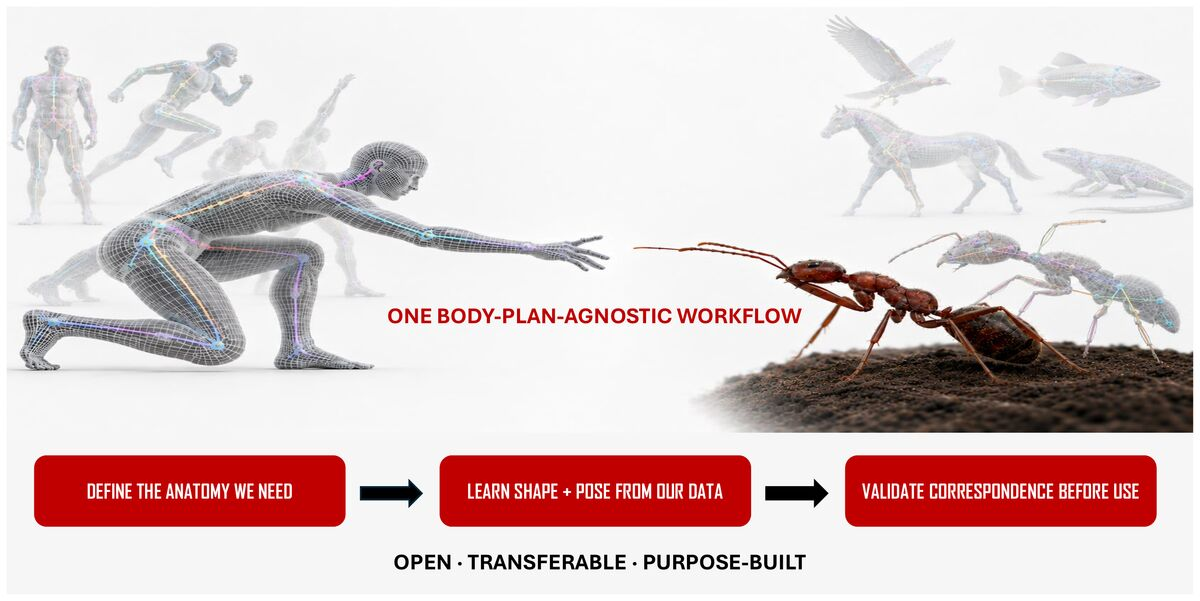
\includegraphics[width=0.58\linewidth]{figures/fig_beyond_ants.jpg}
\caption[Body-plan-agnostic workflow]{The same body-plan-agnostic workflow:
define the anatomy, learn shape and pose from data, validate correspondence
before use.}
\label{fig:beyond-ants}
\end{figure}

\subsection{Limitations}

The scans are incomplete and heterogeneous, the expert benchmark is small (11
specimens), and synthetic targets come from the model and so bound real error
from below. A fixed topology and a 25-dimensional shape basis cannot express
every specimen, and residual deformation is ambiguous with pose. Local
ambiguity, laterality, thin structures and global consistency of the
correspondence are unresolved. Expert annotation has its own uncertainty,
trait definitions are coupled to scale, and population-level validity does not
imply specimen-level validity. Fitting is computationally expensive, and not
all large-corpus results could be reproduced in the final environment.

\subsection{Outlook}

Each direction follows from a diagnosed failure, and none was implemented.
Independent pointwise votes collapse, which calls for a global mechanism:
functional maps~\cite{fmaps} or optimal transport~\cite{ot}, with partial
variants for incomplete scans. The absence of an anatomical signal in the
objective calls for skeleton-conditioned correspondence or a learned 3D joint
predictor; free deformation absorbing pose error calls for structured
deformation; and the synthetic-to-real gap calls for scan-realistic synthetic
training with holes, missing limbs and disconnected components. The most
ambitious direction is an anatomical canonical field that predicts, for every
observed point, its part, joint-relative coordinates, laterality and a
confidence, so that correspondence becomes the mapping of a scan into a
canonical anatomical coordinate system.

\subsection{What the internship taught me}

Technically, the internship taught me to treat an objective as a proxy and to
test the mechanism behind it: I learned to build ground truth, to check it
before trusting it, and to report negative results with the same care as
positive ones. Professionally, it taught me to work on a live shared
repository under review, to fix success criteria before an experiment, to run
reproducible batch experiments on two HPC systems, and to redirect a project
when the evidence contradicts its starting hypothesis, a decision that is only
defensible alongside the evidence that motivated it.
